\documentclass[journal,12pt,twocolumn]{IEEEtran}
\usepackage{graphicx}
\usepackage{paralist}
\usepackage{setspace}
\usepackage{gensymb}
\singlespacing
\usepackage[cmex10]{amsmath}
\usepackage{amsthm}
\usepackage{amsmath}
\usepackage{amssymb}
\usepackage{mathrsfs}
\usepackage{txfonts}
\usepackage{stfloats}
\usepackage{bm}
\usepackage{cite}
\usepackage{cases}
\usepackage{subfig}
\usepackage{longtable}
\usepackage{multirow}

\usepackage{enumitem}
\usepackage{mathtools}
\usepackage{steinmetz}
\usepackage{tikz}
\usepackage{circuitikz}
\usepackage{verbatim}
\usepackage{tfrupee}
\usepackage[breaklinks=true]{hyperref}
\usepackage{graphicx}
\usepackage{tkz-euclide}

\usetikzlibrary{calc,math}
\usepackage{listings}
    \usepackage{color}                                            %%
    \usepackage{array}                                            %%
    \usepackage{longtable}                                        %%
    \usepackage{calc}                                             %%
    \usepackage{multirow}                                         %%
    \usepackage{hhline}                                           %%
    \usepackage{ifthen}                                           %%
    \usepackage{lscape}     
\usepackage{multicol}
\usepackage{chngcntr}

\DeclareMathOperator*{\Res}{Res}

\renewcommand\thesection{\arabic{section}}
\renewcommand\thesubsection{\thesection.\arabic{subsection}}
\renewcommand\thesubsubsection{\thesubsection.\arabic{subsubsection}}

\renewcommand\thesectiondis{\arabic{section}}
\renewcommand\thesubsectiondis{\thesectiondis.\arabic{subsection}}
\renewcommand\thesubsubsectiondis{\thesubsectiondis.\arabic{subsubsection}}


\hyphenation{op-tical net-works semi-conduc-tor}
\def\inputGnumericTable{}                                 %%

\lstset{
%language=C,
frame=single, 
breaklines=true,
columns=fullflexible
}
\begin{document}


\newtheorem{theorem}{Theorem}[section]
\newtheorem{problem}{Problem}
\newtheorem{proposition}{Proposition}[section]
\newtheorem{lemma}{Lemma}[section]
\newtheorem{corollary}[theorem]{Corollary}
\newtheorem{example}{Example}[section]
\newtheorem{definition}[problem]{Definition}

\newcommand{\BEQA}{\begin{eqnarray}}
\newcommand{\EEQA}{\end{eqnarray}}
\newcommand{\define}{\stackrel{\triangle}{=}}
\bibliographystyle{IEEEtran}
\raggedbottom
\setlength{\parindent}{0pt}
\providecommand{\mbf}{\mathbf}
\providecommand{\pr}[1]{\ensuremath{\Pr\left(#1\right)}}
\providecommand{\qfunc}[1]{\ensuremath{Q\left(#1\right)}}
\providecommand{\sbrak}[1]{\ensuremath{{}\left[#1\right]}}
\providecommand{\lsbrak}[1]{\ensuremath{{}\left[#1\right.}}
\providecommand{\rsbrak}[1]{\ensuremath{{}\left.#1\right]}}
\providecommand{\brak}[1]{\ensuremath{\left(#1\right)}}
\providecommand{\lbrak}[1]{\ensuremath{\left(#1\right.}}
\providecommand{\rbrak}[1]{\ensuremath{\left.#1\right)}}
\providecommand{\cbrak}[1]{\ensuremath{\left\{#1\right\}}}
\providecommand{\lcbrak}[1]{\ensuremath{\left\{#1\right.}}
\providecommand{\rcbrak}[1]{\ensuremath{\left.#1\right\}}}
\theoremstyle{remark}
\newtheorem{rem}{Remark}
\newcommand{\sgn}{\mathop{\mathrm{sgn}}}
\providecommand{\abs}[1]{\left\vert#1\right\vert}
\providecommand{\res}[1]{\Res\displaylimits_{#1}} 
\providecommand{\norm}[1]{\left\lVert#1\right\rVert}
%\providecommand{\norm}[1]{\lVert#1\rVert}
\providecommand{\mtx}[1]{\mathbf{#1}}
\providecommand{\mean}[1]{E\left[ #1 \right]}
\providecommand{\fourier}{\overset{\mathcal{F}}{ \rightleftharpoons}}
%\providecommand{\hilbert}{\overset{\mathcal{H}}{ \rightleftharpoons}}
\providecommand{\system}{\overset{\mathcal{H}}{ \longleftrightarrow}}
	%\newcommand{\solution}[2]{\textbf{Solution:}{#1}}
\newcommand{\comb}[2]{{}^{#1}\mathrm{C}_{#2}}
\newcommand{\solution}{\noindent \textbf{Solution: }}
\newcommand{\cosec}{\,\text{cosec}\,}
\newcommand{\cosec}{}
\providecommand{\dec}[2]{\ensuremath{\overset{#1}{\underset{#2}{\gtrless}}}}
\newcommand{\myvec}[1]{\ensuremath{\begin{pmatrix}#1\end{pmatrix}}}
\newcommand{\mydet}[1]{\ensuremath{\begin{vmatrix}#1\end{vmatrix}}}
\numberwithin{equation}{subsection}
\makeatletter
\@addtoreset{figure}{problem}
\makeatother
\let\StandardTheFigure\thefigure
\let\vec\mathbf
\renewcommand{\thefigure}{\theproblem}
\def\putbox#1#2#3{\makebox[0in][l]{\makebox[#1][l]{}\raisebox{\baselineskip}[0in][0in]{\raisebox{#2}[0in][0in]{#3}}}}
     \def\rightbox#1{\makebox[0in][r]{#1}}  
     \def\centbox#1{\makebox[0in]{#1}}
     \def\topbox#1{\raisebox{-\baselineskip}[0in][0in]{#1}}
     \def\midbox#1{\raisebox{-0.5\baselineskip}[0in][0in]{#1}}
\vspace{3cm}
\title{Assignment 3}
\author{Gaureesha Kajampady - EP20BTECH11005}
\maketitle  
\newpage
\bigskip
\renewcommand{\thefigure}{\theenumi}
\renewcommand{\thetable}{\theenumi}
Download all python codes from 
\begin{lstlisting}
https://github.com/gaureeshk/assignment2/blob/main/Codes/assignment3.py
\end{lstlisting}
%
and latex-tikz codes from 
%
\begin{lstlisting}
https://github.com/gaureeshk/assignment2/blob/main/assignment3.tex
\end{lstlisting}
\section{Problem}
A random variable X has probability density function f(x) as shown below:
\begin{enumerate}
f(x)=\begin{cases}
          a+bx \quad &\text{for} \,\, 0<x<1 \\
          0 \quad  &\text{otherwise} \\
     \end{cases}
\end{enumerate}
If the expected value $E\left[X\right]=2/3$, then \pr{X<0.5} is \rule{2cm}{0.15mm}
\section{Solution}
Since the total probabilty is 1,\\
\begin{align}
\int_{-\infty}^{\infty}f(x)dx=1 \\
\implies \int_{0}^{1}f(x)dx=1 \\
\implies a+\frac{b}{2}=1 \label{eq1}
 \end{align}
 Also,
 \begin{align}
     E[X]=\int_{-\infty}^{\infty}xf(x)dx\\
     \frac{2}{3}=\int_{0}^{1}(ax+bx^{2})dx\\
     \implies \frac{a}{2}+\frac{b}{3}=\frac{2}{3}\label{eq2}
\end{align}
using \eqref{eq1} and \eqref{eq2} we get,\\
\begin{align}
\begin{bmatrix}
1 & \frac{1}{2}\\
\frac{1}{2} & \frac{1}{3}
\end{bmatrix}
\begin{bmatrix}
a\\
b
\end{bmatrix}
=\begin{bmatrix}
1\\
\frac{2}{3}
\end{bmatrix}\\
\implies 
\begin{bmatrix}
a\\
b
\end{bmatrix}
=\begin{bmatrix}
1 & \frac{1}{2}\\
\frac{1}{2} & \frac{1}{3}
\end{bmatrix}^{-1}
\begin{bmatrix}
1\\
\frac{2}{3}
\end{bmatrix}
=\begin{bmatrix}
0\\
2
\end{bmatrix}
\end{align}
Hence a=0 and b=2.
\begin{align}
F_{X}(x)&=\int_{-\infty}^{x}f(x)dx.\\
        &=\begin{cases}
        0 \quad &\text{for}\,\, x\leq0\\
        x^{2} \quad &\text{for}\,\, 0<x<1\\
        1 \quad &\text{for} \,\, x\geq1
               \end{cases}\\
\hence \pr{X<0.5}&=F_{X}(0.5)=0.25
\end{align}
Hence the required probability is 0.25.\\\\
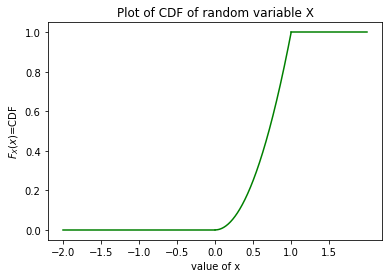
\includegraphics[width=0.5\textwidth]{assignment3.png}
\end{document}





















